\documentclass[a4paper,10pt]{article}
\usepackage[english]{babel}
\usepackage[utf8]{inputenc}
\usepackage{url}
\usepackage[margin=1in]{geometry}
\usepackage{enumitem}

\setlist[itemize]{leftmargin=1.2in}


\usepackage[nottoc]{tocbibind}
\usepackage{fancyvrb} 
\usepackage{float}
\usepackage{graphicx}
\usepackage{subcaption}
\usepackage{color}
\usepackage{booktabs}
\usepackage{listings}

\title{Combinatorial Optimization\\Homework 1 – Knapsack Problem}
\author{Matyáš Skalický\\skalimat@fit.cvut.cz}

\begin{document}
\maketitle
\tableofcontents
\medskip


\section{Implementation}
The brute-force solver of the knapsack problem was implemented using the recursive approach. The solver was implemented in Python. To speed the experiments up, they were executed in parallel to fully utilize the CPU. The datasets were subsampled from 500 to 250 samples to speed up the experiments.

The naive brute-force search recursively enumerates all possible solutions until a feasible solution is found, or the solution space exhausted.

An optimized branch\&bound solver was also implemented and compared to the naïve brute-force approach. It utilizes several speedups:

\begin{enumerate}[leftmargin=1in]
	\item[\emph{exceeded weight}] Weight of the bag already exceeds the capacity of the bag. Do not recurse further.
	\item[\emph{residuals mincost}] Sum the cost of remaining items that can be added into the bag. Do not recurse further \lstinline{if (cost + residual) < mincost} where \emph{mincost} is the decision version requirement.
\end{enumerate}

\clearpage

\section{Experiments}
\subsection{Instance Size}
First, let's compare the algorithms on a mixed dataset (half from the NR and half from the ZR dataset). Figure \ref{size_vs_ops_boxplot} shows that the number of performed operations grows exponentially with the size of the instance.

\begin{figure}[!htb]
	\centering
  	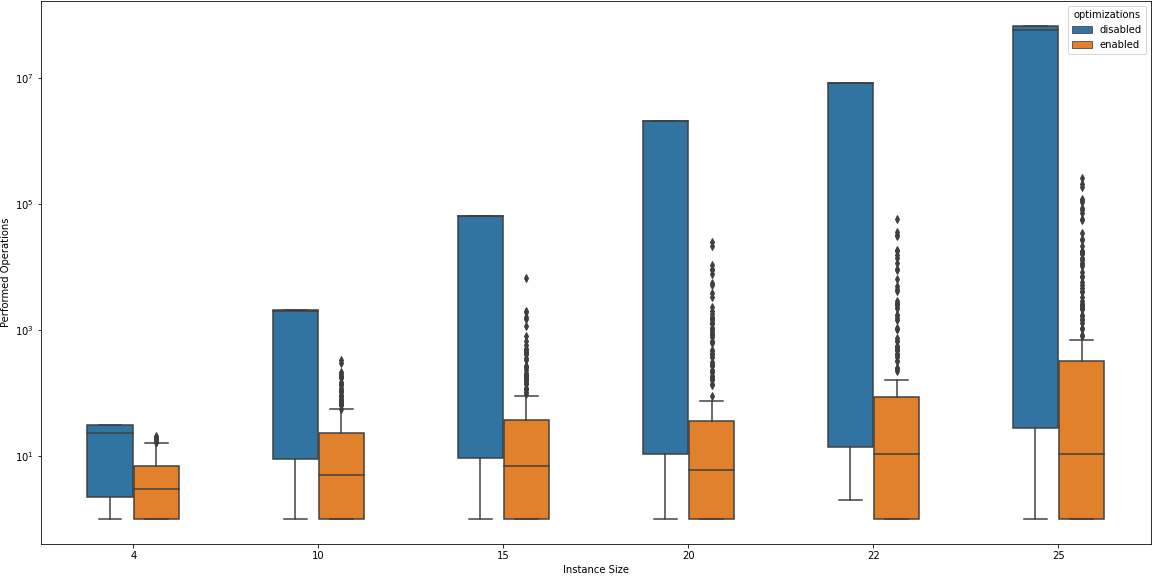
\includegraphics[width=\textwidth]{size_vs_performed_boxplot.png}
	\caption{Instance size vs. number of performed operations}
	\label{size_vs_ops_boxplot}
\end{figure}

Let's break down the number of operations by the dataset. Figure \ref{size_vs_ops_lineplot} compares the required number of operations by dataset and also by solver. We can see, that when branch\&bound is disabled, the complexity is the same for both datasets. When we enable the branch\&bound, the speedup is most notable for the \emph{NR} dataset.

\begin{figure}[!htb]
	\centering
  	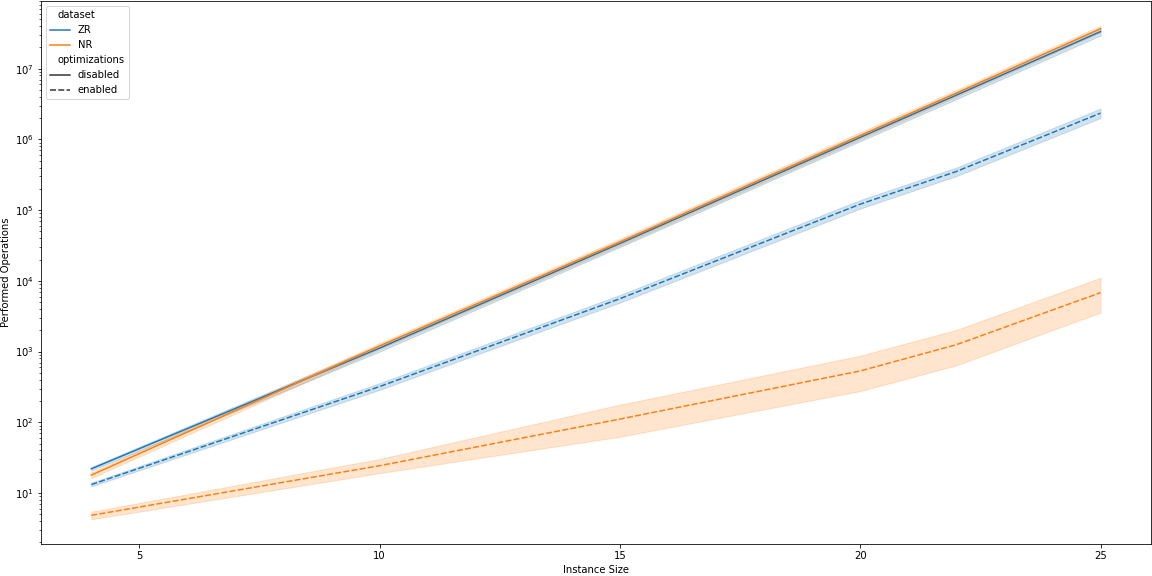
\includegraphics[width=\textwidth]{size_vs_ops_lineplot.png}
	\caption{Instance size vs. number of performed operations by dataset}
	\label{size_vs_ops_lineplot}
\end{figure}

\clearpage

\subsection{Histogram}
Following Figure \ref{size_20_hist} highlights the finding, that the branch\&bound algorithm speedup significance was accented mainly on the NR dataset.

\begin{figure}[!htb]
	\centering
  	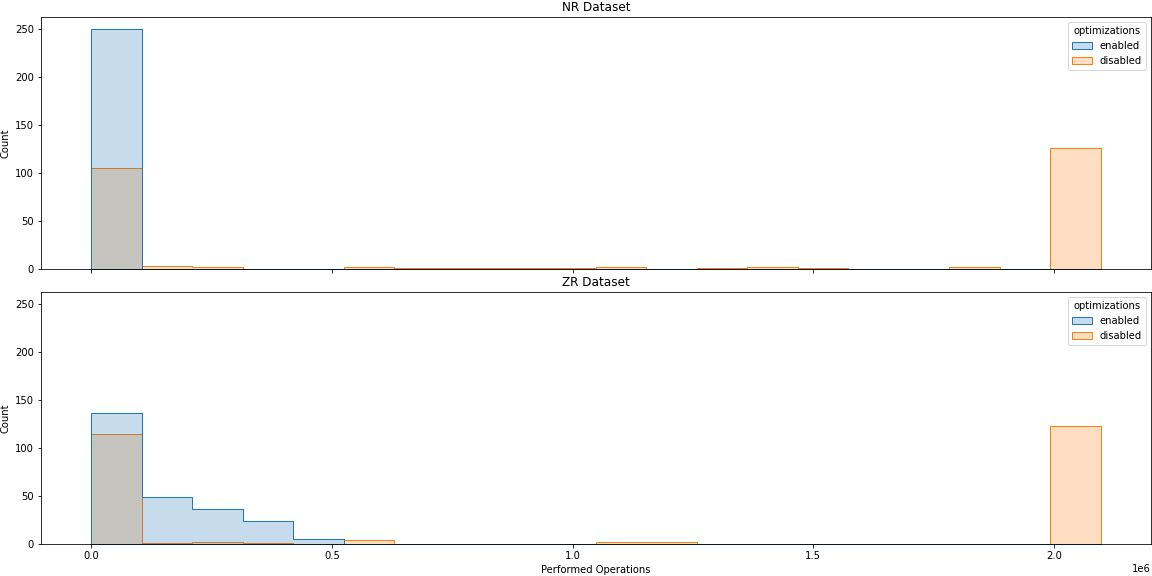
\includegraphics[width=\textwidth]{size_20_hist.png}
	\caption{Histogram for number of operations; breakdown by dataset type and optimizations}
	\label{size_20_hist}
\end{figure}


\section{Discussion}
The \emph{ZR} dataset is most-likely designed in a way to combat the usage of branch\&bound speedups. My assumption was, that the branch\&bound technique will be more effective, but overall, it should grow asymptotically with the brute-force approach. 

When the optimizations were disabled, the computational cost was almost identical for the both methods (best seen on Figure \ref{size_20_hist}). When using the branch\&bound technique, there was a significant difference between the provided datasets as the \emph{ZR} dataset forced the solver to often explore all possible solutions.

Since we are using a decision version of the knapsack problem, without branch\&bound we need to explore all the possible solutions before saying that there isn't one. This is clearly visible on the right side of the Figure \ref{size_20_hist}.

\end{document}